\documentclass{article}
\usepackage{titling}
\newcommand{\subtitle}[1]{\posttitle{\par\end{center}\begin{center}\large#1\end{center}\vskip0.5em}}
\usepackage[left=1.5cm, right=1.5cm, top=1.5cm, bottom=1.5cm]{geometry}
\usepackage{graphicx, float}
\usepackage[font=footnotesize,labelfont=bf,belowskip=0pt,aboveskip=2pt]{caption}
\usepackage[hidelinks]{hyperref}
\usepackage{fixltx2e}
\usepackage{amsmath,amssymb,mathrsfs}
\usepackage{sidecap}
\usepackage{gensymb}
\setlength\parindent{0pt}
\renewcommand{\floatpagefraction}{.8}
\pagenumbering{gobble}
\usepackage[labelsep=period]{caption}
\usepackage[skip=8pt]{caption}
\renewcommand{\figurename}{}
\renewcommand{\thefigure}{\small{Figure~S\arabic{figure}}}
\sidecaptionvpos{figure}{t}
\usepackage{fontspec}
\setmainfont{Calibri}
\usepackage{atbegshi}
\begin{document}

\renewcommand{\figurename}{\small{Figure}}

\renewcommand{\thefigure}{S1}
\begin{figure}[H]
\centering
\makebox[\textwidth][c]{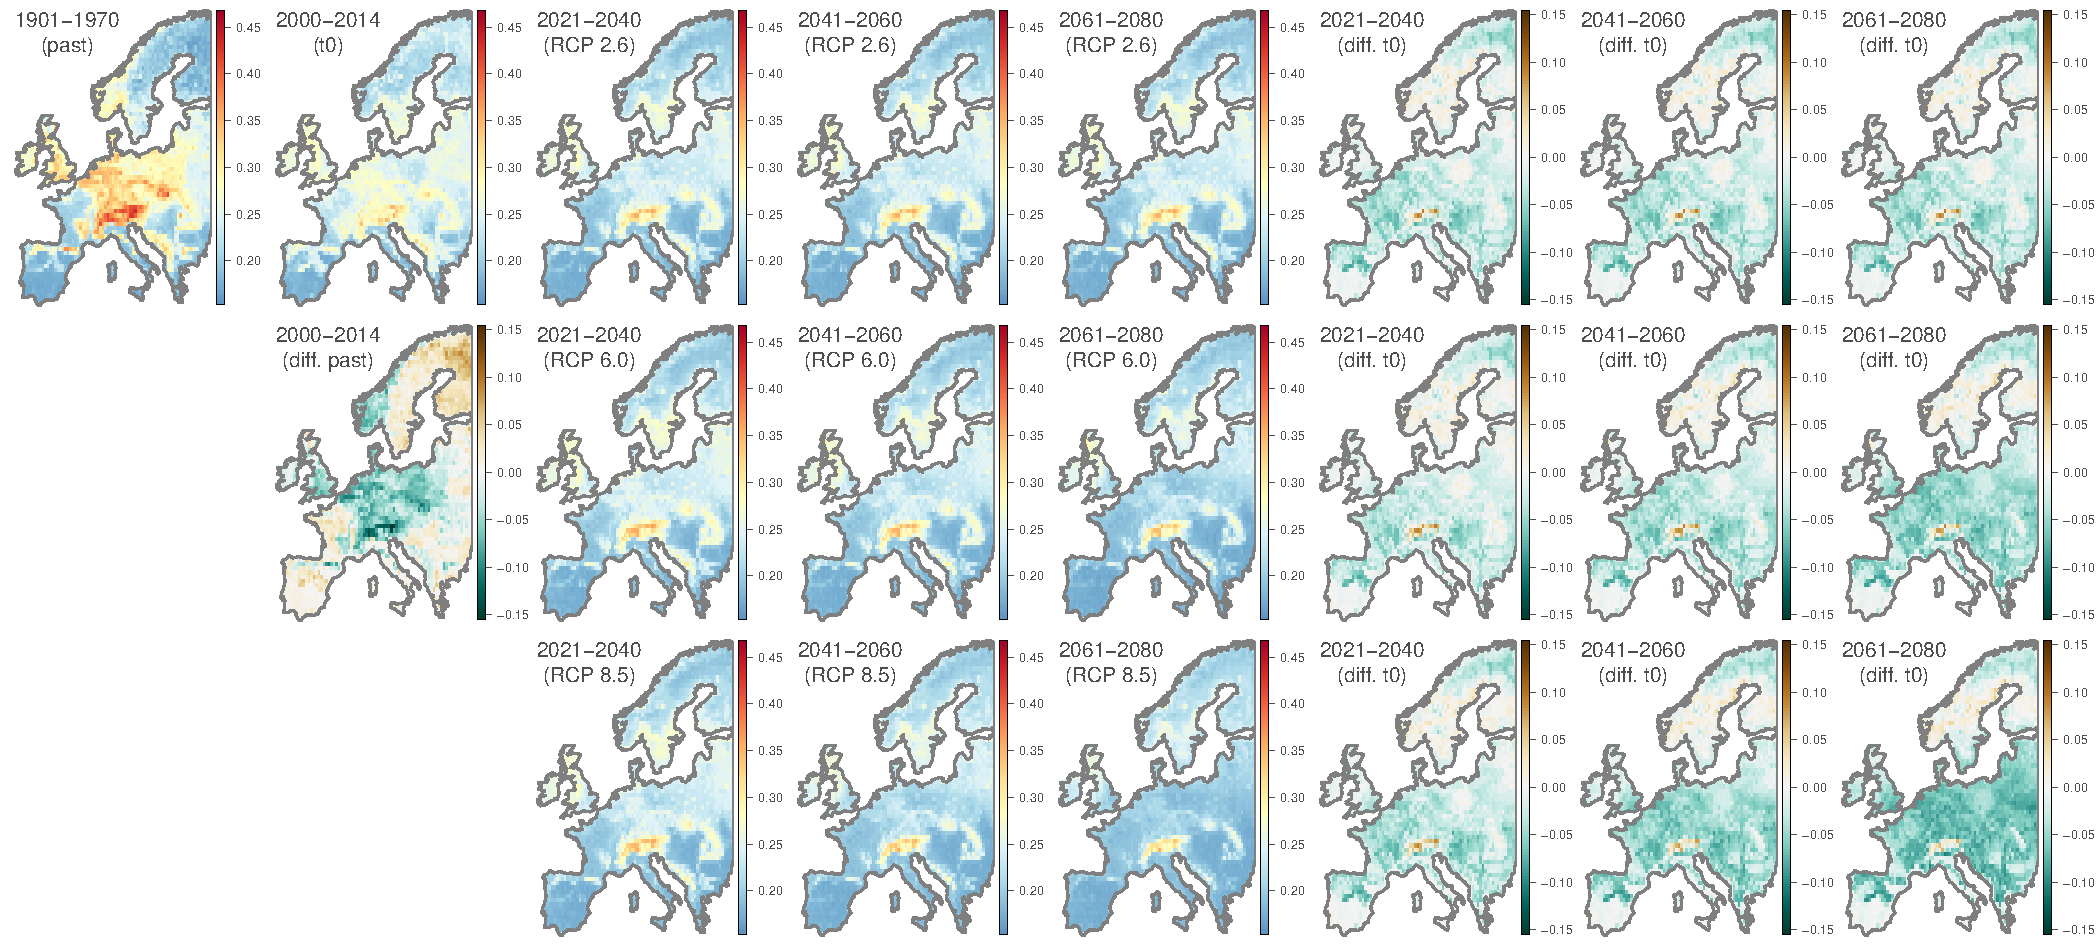
\includegraphics[width=1.00\textwidth]{Bombus_ESI_diffrences.pdf}}
\caption{\small{\textbf{1� environmental variable involved in ecological niche modelling: air temperature near surface (�C).}
We here also report the difference between each future estimate and the estimate for the current period (t0).}}
\label{FigureS1}
\end{figure}

\renewcommand{\thefigure}{S2}
\begin{figure}[H]
\centering
\makebox[\textwidth][c]{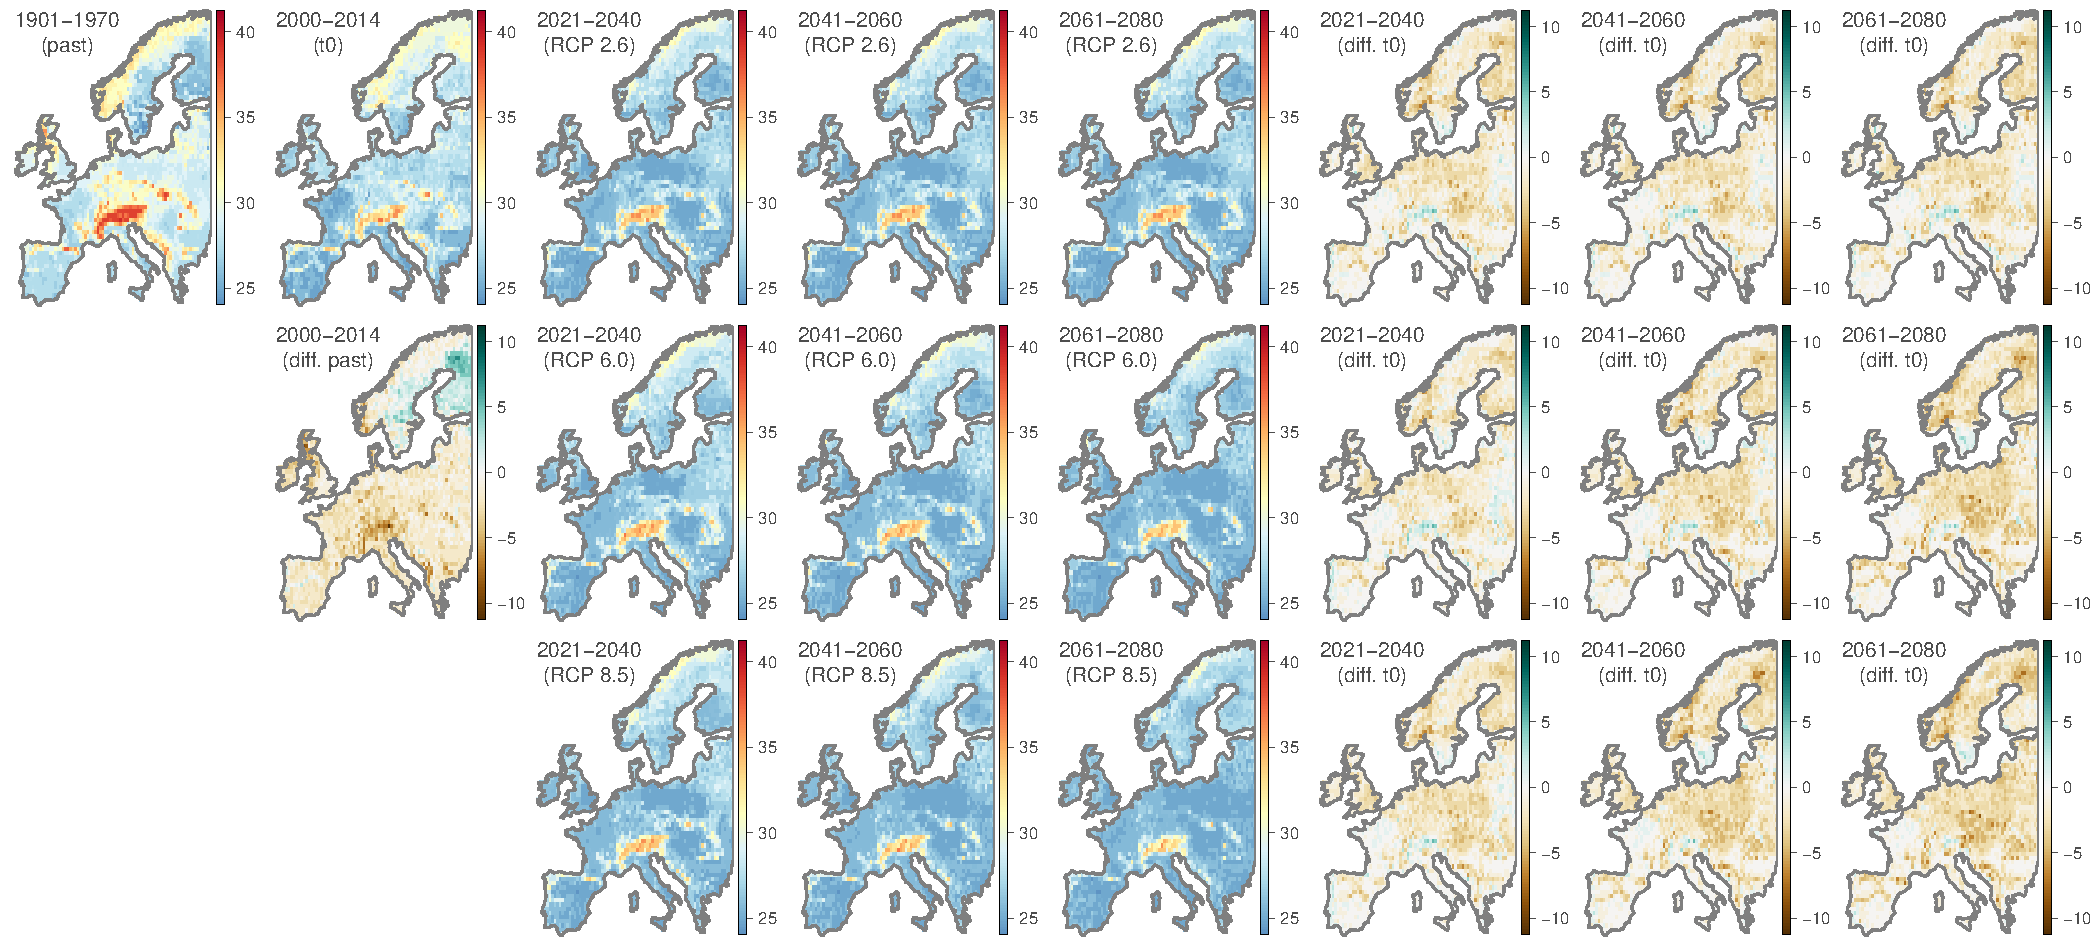
\includegraphics[width=1.00\textwidth]{Bombus_SRI_diffrences.pdf}}
\caption{\small{\textbf{2� environmental variable involved in ecological niche modelling: precipitation (kg/m\textsuperscript{2}/day).}
We here also report the difference between each future estimate and the estimate for the current period (t0).}}
\label{FigureS2}
\end{figure}

\end{document}
